\chapter{Introduction}

\pagebreak

\section{The State of Mental Health}

Burden of mental disorders had risen over last few decades. Mental health is a state of well-being in which the individual realizes his or her own abilities, can cope with the normal stresses of life, can work productively and is able to make a contribution to his or her community. WHO estimated that globally over 450 million people suffer from mental disorders. Currently mental and behavioural disorders account for about 12 percent of the global burden of diseases. Major proportions of mental disorders come from low and middle income countries.

\begin{figure}[H]
    \centering
    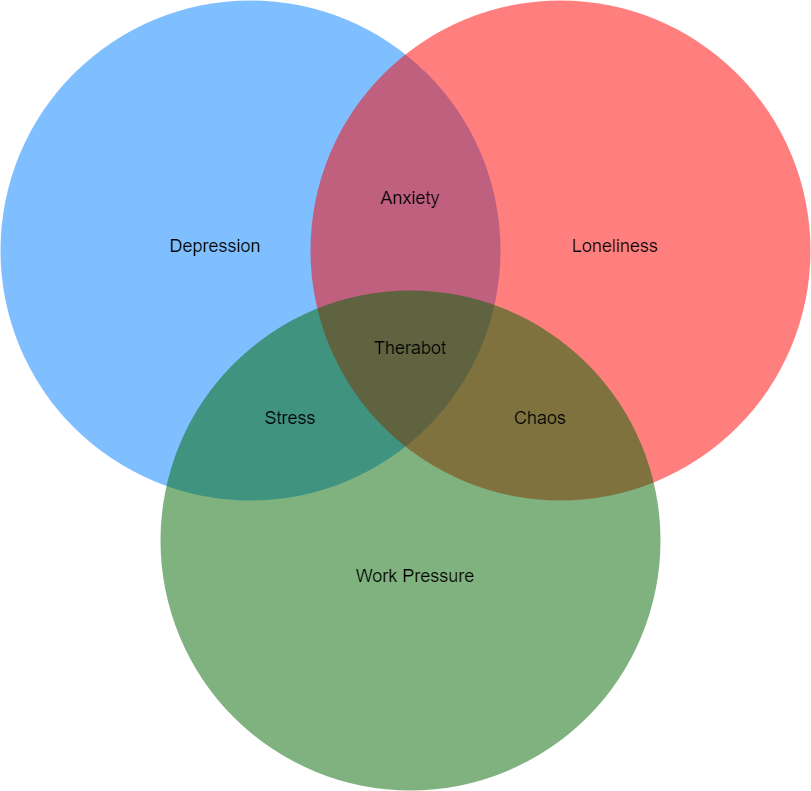
\includegraphics[width=6cm]{images/roots-mental-health-issues.png}
    \caption{Roots of Mental Health Issues}
    \label{fig:roots-mental-health-issues}
\end{figure}

Progress in mental health service delivery has been slow in most low- and middle-income countries. Barriers include the existing public-health priorities and its influence on funding; challenges to delivery of mental health care in primary-care settings; the low numbers of those trained in mental health care; and the lack of mental health perspective in public-health leadership. There have been numerous calls for invoking political will, for enhancing advocacy and for galvanizing community participation; all with scant improvement in outcomes.

Thus, it becomes now opportune to explore the paradigm of mental health awareness as a means of combating stigma, enhancing prevention, ensuring early recognition, and also stimulating simple and practical interventions within the community. Today there are opportunities in terms of growing acknowledgement of mental disorders as key targets of global health action, as well as of leveraging new technologies particularly internet, big data and cell phones in amplifying simple field interventions found successful in primary care and other echelons.

\pagebreak

\section{The Cognitive Behavioural Therapy}

Cognitive behavioral therapy (CBT) is a short-term therapy technique used by counselors and therapists to teach individuals to change their unwanted behaviors by changing their thought patterns. The premise of cognitive behavioral therapy is that our thought patterns (cognition) and interpretations of life events greatly influence how we behave and, ultimately, how we feel.

\begin{figure}[H]
    \centering
    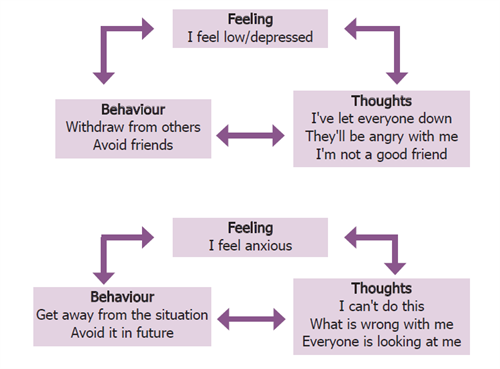
\includegraphics[width=8cm]{images/cbt-diagram.jpg}
    \caption{Sequence of Cognitive Behavioural Therapy}
    \label{fig:cbt-diagram}
\end{figure}

CBT is a form of psychotherapy that focuses on how your thoughts, beliefs and attitudes affect your feelings and behavior. It aims to teach you effective coping strategies for dealing with different problems throughout life. CBT can help you make sense of overwhelming problems by breaking them down into smaller parts.

One of the key tenets of CBT is that distorted thinking leads to distress and problematic behaviors, whereas thinking realistically with less negativity allows individuals to respond to challenging life circumstances in an effective way. Research shows this technique is an effective therapy for not only depression and panic disorder, but many illnesses and dysfunctional behaviors.

\pagebreak

\section{The Rise of Chatbots}

A chatbot is one of the simple ways to transport data from a computer without having to think for proper keywords to look up in a search or browse several web pages to collect information; users can easily type their query in natural language and retrieve information. In this paper, information about the design, implementation of the chatbot has been presented.

From the survey above, it can be said that the development and improvement of chatbot design grow at an unpredictable rate due to variety of methods and approaches used to design a chatbot. Chatbot is a great tool for quick interaction with the user. They help us by providing entertainment, saving time and answering the questions that are hard to find. The Chatbot must be simple and conversational. Since there are many designs and approaches for creating a chatbot, it can be at odds with commercial considerations. Researchers need to interact and must agree on a common approach for designing a Chatbot.

In this project, we looked into how chatbots are developed and the applications of chatbots in various fields. In addition, comparison has been made with other chatbots in the same field of interest. A general purpose chatbot must be simple, user friendly, must be easily understood and the knowledge base must be compact. Although some of the commercial products have recently emerged, improvements must be made to find a common approach for designing a chatbot.

Chatbots have seen a huge rise in the recent markets and have primarily been used in the fields of service, question and answering and quite recently, home automation. They have proven to be very useful in the field of automation and have successfully replaced menial jobs that could’ve cost a lot of money for major corporations. Current commercial chatbots are capable of understanding simple sentences through pattern matching techniques, and search for questions asked in a repository of answers. This works out well in a closed scenario where the kind of questions the user may ask are limited, but not in a real life scenario.

\begin{figure}[H]
    \centering
    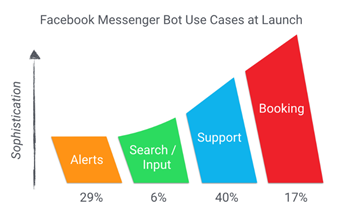
\includegraphics[width=8cm]{images/chatbot-usecases.png}
    \caption{Usecases of Chatbots}
    \label{fig:chatbot-usecases}
\end{figure}

Chatbots were later trained on neural networks to become much smarter, using a larger dataset. They were trained to learn on a wider spectrum and can understand sentences in a more humane form due to the advancements in NLP. But with all the new things that chatbots now have to learn, they’ve never really been personal to an individual.

\begin{figure}[H]
    \centering
    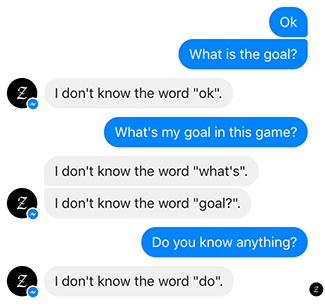
\includegraphics[width=8cm]{images/dumb-chatbot.png}
    \caption{Dumb Chatbots}
    \label{fig:dumb-chatbot}
\end{figure}

The objective of our method is to create a personalized user model that is unique to every user but keeps them anonymous at the same time. This helps the chatbot response generator understand who the user is and push relatable content and context when necessary.

\pagebreak

\section{The Abstract of Artificial Intelligence}

Artificial Intelligence (AI) is defined as intelligence exhibited by an artificial entity to solve complex problems and such a system is generally assumed to be a computer or machine. Artificial Intelligence is an integration of computer science and physiology Intelligence in simple language is the computational part of the ability to achieve goals in the world. Intelligence is the ability to think to imagine creating memorizing and understanding, recognizing patterns, making choices adapting to change and learn from experience.

\begin{figure}[H]
    \centering
    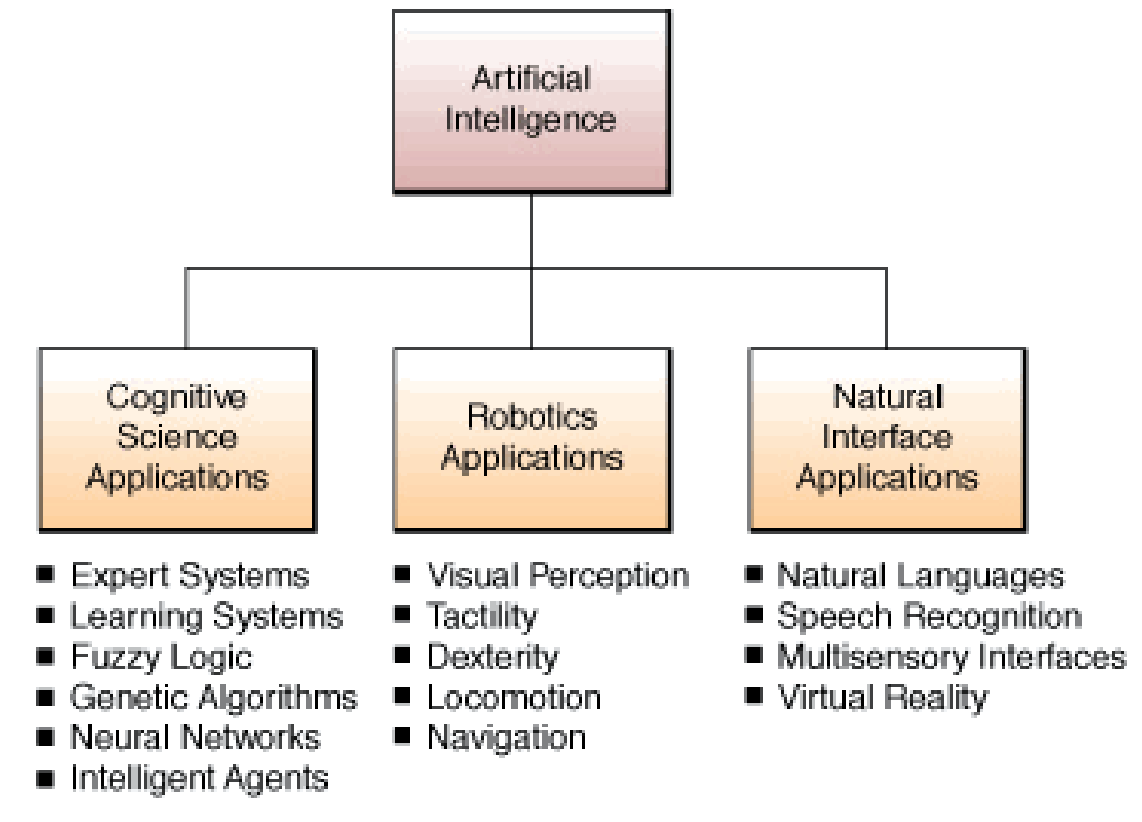
\includegraphics[width=10cm]{images/ai-overview.png}
    \caption{Overview of Artificial Intelligence}
    \label{fig:ai-overview}
\end{figure}

Artificial Intelligence was created with the sole aim of mimicking or even outperforming human minds. Thus it is very important we question the fact whether it has actually been able to do so.

It cannot be ignored that the fact of AI is being used all around us especially in the fields of medicine, robotics, law, stock trading etc. It is being used in homes and big establishments. such as military bases and the NASA space station. NASA has sent out artificially intelligent robots to planets so as to learn more about their habitat and atmosphere, with the intention of investigating if there is a possibility of humans living on these planets.

Expert systems have been used by Mercedes Benz and other auto manufacturers in the design of vehicle components, subway systems in Washington, D.C. use expert system software controllers to cause subway trains to stop within 3 inches of the right spot on the platform. These trains have motormen primarily to reassure passengers. AI has filtered into general applications in these fields and has become so common that it is not referred to as Artificial Intelligence anymore.

Blind supporters of AI would point to the time when AI Deep Blue II defeated chess master Garry Kasparov to prove that Artificial Intelligence can in fact be smarter than humans. Though there is no doubt that the AI Deep Blue II won that game, it is still probably one of the dumbest software alive. The operators were programming the AI in every round depending on the opposition’s last move. Also, the Deep Blue II had studied all of Kasparov’s previous games while the latter wasn’t given the same benefit. One can safely say that even though the Deep Blue II AI defeated Kasparov, it was never a fair fight to begin with. Latest technologies like Xbox 360’s Kinect and iPhone’s Siri use algorithms based on Artificial Intelligence, but it is a well-known fact that these technologies are a long way from being perfect.

Thus we can safely conclude that though Artificial Intelligence has made a lot of progress in the past few decades, it is not at a level where in one can confidently state that it is now ready to completely replace the human mind. That being said, large scale research is now being conducted into the field of proper simulation of the human brain.
